To help with debugging and automate parts of the analysis process, a web app was developed to interact with data collected during runs.
The key feature is a parser for the log files generated during agent runs. This allows for filtering important events and displaying them chronologically, as well as automatically collecting statistics.
Such key events are when a new level is loaded, when a shot is planned and executed and when new \ac{CBR} cases are added or evaluated.

Because all relevant information is logged during the run, this also allows one to view other shot candidates apart from the one that was performed.
For \ac{CBR} based shots, the information about expected and actual effects can be used to render an overlay of those objects on top of the scene.
This allows manual analysis of cases that were applied to a situation and comparing the effects.
However, because intermediary situation files have not been recorded, this only works for the first shot of a given level.

\begin{figure}[H]%
    \begin{center}%
        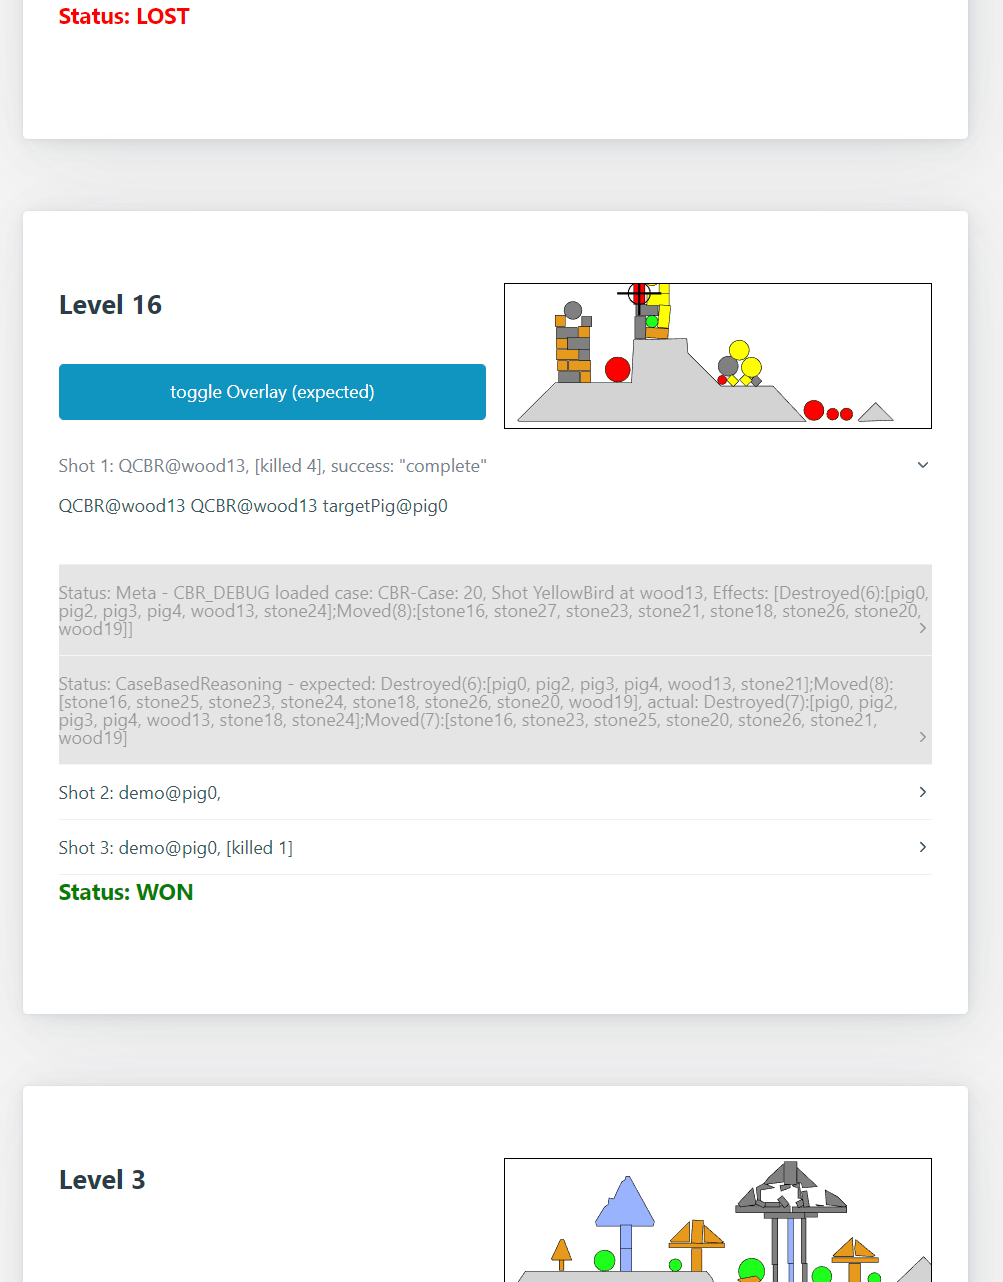
\includegraphics[width=15cm]{data/run_analysis2}%
        \vskip -0.3cm%
        \caption{Screenshot from the Analysis tool, showing a filtered chronology of a run. Level 16 Shot 1 shows both considered and chosen strategies as well as the overlay of expected effects}%
        \vskip -0,2cm%
        \label{fig:run-analysis}%
    \end{center}%
\end{figure}%

Additional features are the rendering of arbitrary levels or situations, which can then be manipulated, i.e. objects can be deleted, duplicated or moved.
This can either be used to test relations between objects or to export the data for use with the prolog planning module.
